\documentclass[11pt,a4paper]{article}

% ==============================================================================
%  MANUAL DE USO  ·  Captura de osciloscopio Siglent (USB/SCPI) -> CSV
%  Direccion de Docencia Experimental · Facultad de Ciencias · U. de Chile
%  Diseno: minimalista, escala de grises (mismo estilo que guia_rlc.tex)
% ==============================================================================

\usepackage[utf8]{inputenc}
\usepackage[T1]{fontenc}
\usepackage[a4paper,margin=2.6cm,top=2.4cm,bottom=2.4cm]{geometry}
\usepackage{amsmath,amssymb}
\usepackage{siunitx}
\usepackage{graphicx}
\usepackage{xcolor}
\usepackage{tikz}
\usepackage{enumitem}
\usepackage{titlesec}
\usepackage{fancyhdr}
\usepackage{tcolorbox}
\usepackage{booktabs}
\usepackage{listings}
\usepackage{hyperref}

\usetikzlibrary{calc,positioning,arrows.meta}
\tcbuselibrary{skins}

% ---- Paleta en escala de grises ----------------------------------------------
\definecolor{gtinta}{gray}{0.13}   % texto principal
\definecolor{gmedio}{gray}{0.45}   % secundario
\definecolor{gsuave}{gray}{0.72}   % lineas finas
\definecolor{gcaja}{gray}{0.96}    % fondo de cajas
\definecolor{gborde}{gray}{0.80}   % borde de cajas

\color{gtinta}

% ---- Tipografia de titulos ---------------------------------------------------
\titleformat{\section}
  {\normalfont\large\bfseries\color{gtinta}}
  {\thesection}{0.7em}{}[\vspace{2pt}\color{gsuave}\titlerule]
\titleformat{\subsection}
  {\normalfont\normalsize\bfseries\color{gtinta}}
  {\thesubsection}{0.6em}{}
\titlespacing*{\section}{0pt}{1.4em}{0.7em}
\titlespacing*{\subsection}{0pt}{1.0em}{0.4em}

% ---- Encabezado y pie --------------------------------------------------------
\pagestyle{fancy}
\fancyhf{}
\renewcommand{\headrulewidth}{0.4pt}
\renewcommand{\footrulewidth}{0pt}
\fancyhead[L]{\footnotesize\color{gmedio}Captura de osciloscopio Siglent · Manual de uso}
\fancyhead[R]{\footnotesize\color{gmedio}DDE · Facultad de Ciencias · U. de Chile}
\fancyfoot[C]{\footnotesize\color{gmedio}\thepage}

% ---- Caja de nota ------------------------------------------------------------
\newtcolorbox{nota}[1][]{
  enhanced, colback=gcaja, colframe=gborde, boxrule=0.4pt,
  arc=1.5pt, left=8pt, right=8pt, top=6pt, bottom=6pt,
  fonttitle=\bfseries\small, coltitle=gtinta, #1}

% ---- Caja de advertencia (mismo gris, marcada con barra) ---------------------
\newtcolorbox{aviso}{
  enhanced, colback=white, colframe=gtinta, boxrule=0pt,
  leftrule=2.5pt, arc=0pt, left=8pt, right=8pt, top=6pt, bottom=6pt}

\setlist[itemize]{leftmargin=1.3em, itemsep=2pt, topsep=3pt}
\setlist[enumerate]{leftmargin=1.5em, itemsep=4pt, topsep=3pt}

\sisetup{detect-all, separate-uncertainty=true, range-phrase={ a }}

\lstdefinestyle{consola}{
  basicstyle=\ttfamily\small\color{gtinta},
  backgroundcolor=\color{gcaja},
  frame=single, rulecolor=\color{gborde}, framesep=5pt,
  breaklines=true, showstringspaces=false, columns=fullflexible
}
\lstset{style=consola}

\hypersetup{colorlinks=true, linkcolor=gtinta, urlcolor=gtinta, citecolor=gtinta}

% ==============================================================================
\begin{document}

% ---- Portada compacta --------------------------------------------------------
\begin{center}
  {\Large\bfseries Captura de osciloscopio Siglent por USB}\\[2pt]
  {\large Manual de uso para proyectos de laboratorio}\\[10pt]
  {\color{gmedio}\rule{0.45\textwidth}{0.4pt}}\\[8pt]
  {\small\color{gmedio}Herramienta de propósito general · Licenciatura en Física}\\[2pt]
  {\footnotesize\color{gmedio}Dirección de Docencia Experimental — Facultad de Ciencias — Universidad de Chile}
\end{center}
\vspace{0.6em}

% ---- Objetivo ----------------------------------------------------------------
\section{Objetivo}
Este manual explica cómo usar \texttt{capturar\_osciloscopio.py}, una
herramienta que descarga una traza (voltaje en función del tiempo) desde un
osciloscopio Siglent conectado por USB y la guarda en un archivo CSV simple,
listo para analizar con Python, MATLAB, Excel o lo que uses en tu informe.

\begin{nota}[title=¿Para qué proyectos sirve?]
Para cualquier experimento donde midas una señal transitoria con el
osciloscopio y necesites los datos crudos: carga/descarga de un capacitor,
respuesta de un sensor óptico, una señal de un acelerómetro, un pulso único
de cualquier tipo. El script no asume nada sobre el origen físico de la
señal --- solo descarga lo que el osciloscopio tenga en pantalla.
\end{nota}

% ---- Alcance ------------------------------------------------------------------
\section{Alcance}
\begin{itemize}
  \item Soporta osciloscopios \textbf{Siglent serie SDS1000(CNL+)} (probado
        en un SDS1102CNL+) que hablan el protocolo SCPI sobre USBTMC.
  \item Captura \textbf{un canal a la vez} (\texttt{C1}, \texttt{C2}, etc.).
  \item Pensado para disparo único (\texttt{SINGLE}); también puede leer una
        traza ya detenida en pantalla.
  \item No soporta otras marcas de osciloscopio (Tektronix, Rigol,
        Keysight) ni protocolos distintos de SCPI/USBTMC.
\end{itemize}

% ---- Requisitos ---------------------------------------------------------------
\section{Requisitos}

\subsection{Hardware}
\begin{itemize}
  \item Osciloscopio Siglent serie SDS1000(CNL+).
  \item Cable USB tipo B (el que normalmente trae el instrumento).
  \item Computador con Linux (el procedimiento de permisos de este manual es
        específico de Linux; en Windows/macOS la conexión USBTMC funciona
        distinto).
\end{itemize}

\subsection{Software}
\begin{itemize}
  \item Python 3.9 o superior.
  \item Paquetes: \texttt{numpy}, \texttt{pyvisa}, \texttt{pyvisa-py},
        \texttt{pyusb} (listados en \texttt{requirements.txt}).
\end{itemize}

% ---- Instalacion ---------------------------------------------------------------
\section{Instalación}

\subsection{Entorno de Python}
\begin{lstlisting}
python3 -m venv venv
source venv/bin/activate
pip install -r requirements.txt
\end{lstlisting}

\subsection{Permisos USB}
Linux no permite acceder a dispositivos USB sin privilegios de administrador
a menos que exista una regla que lo autorice explícitamente.

\begin{lstlisting}
sudo cp 99-usbtmc-siglent.rules /etc/udev/rules.d/
sudo groupadd -f usbtmc
sudo usermod -aG usbtmc "$USER"
sudo udevadm control --reload-rules
sudo udevadm trigger
\end{lstlisting}

\begin{aviso}
\textbf{Paso que se olvida con frecuencia.} Después de ejecutar lo anterior,
\emph{cierra sesión y vuelve a entrar} (o reinicia) para que el cambio de
grupo tenga efecto, y \emph{desconecta y reconecta} el cable USB del
osciloscopio. Si no haces ambas cosas, seguirás viendo error de permisos
aunque la regla esté instalada correctamente.
\end{aviso}

\subsection{Verificación}
Con el osciloscopio encendido y conectado:
\begin{lstlisting}
python capturar_osciloscopio.py --help
\end{lstlisting}
Si aparece el mensaje de ayuda sin errores, la instalación está completa.

% ---- Como funciona --------------------------------------------------------
\section{Cómo funciona}
\begin{center}
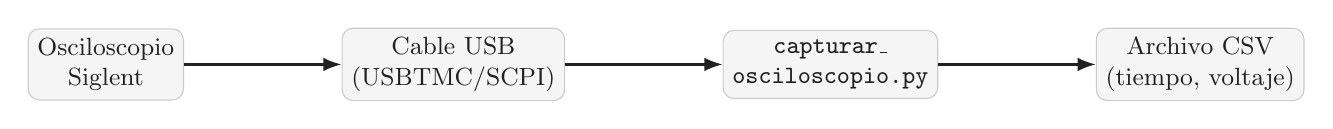
\begin{tikzpicture}[node distance=0.5cm, font=\small,
    every node/.style={draw=gborde, rounded corners, align=center, fill=gcaja, text=gtinta}]
  \node (osc) {Osciloscopio\\Siglent};
  \node[right=2.0cm of osc] (usb) {Cable USB\\(USBTMC/SCPI)};
  \node[right=2.0cm of usb] (script) {\texttt{capturar\_}\\\texttt{osciloscopio.py}};
  \node[right=2.0cm of script] (csv) {Archivo CSV\\(tiempo, voltaje)};
  \draw[-Latex, thick, gtinta] (osc) -- (usb);
  \draw[-Latex, thick, gtinta] (usb) -- (script);
  \draw[-Latex, thick, gtinta] (script) -- (csv);
\end{tikzpicture}
\end{center}
\vspace{0.3em}
El script: (1) se conecta al instrumento, (2) arma un disparo \texttt{SINGLE}
y espera a que el osciloscopio capture, (3) le pregunta la escala vertical y
horizontal que está usando, (4) descarga los puntos crudos de la pantalla y
los convierte a voltios y segundos usando esa escala, y (5) los guarda en el
CSV.

% ---- Uso ------------------------------------------------------------------
\section{Uso}

\begin{center}
\begin{tabular}{@{}lll@{}}
\toprule
\textbf{Comando} & \textbf{Canal} & \textbf{Archivo de salida} \\
\midrule
\texttt{python capturar\_osciloscopio.py} & \texttt{C1} (por defecto) & \texttt{traza\_real.csv} (por defecto) \\
\texttt{python capturar\_osciloscopio.py C2 datos.csv} & \texttt{C2} & \texttt{datos.csv} \\
\texttt{... --sin-disparo} & el que esté activo & no rearma el disparo \\
\bottomrule
\end{tabular}
\end{center}

\vspace{0.4em}
Salida esperada en la terminal:
\begin{lstlisting}
Conectado: Siglent Technologies,SDS1102CNL+,...
20480 puntos capturados en C1.
Ventana: -20.48 us a 184.30 us
Guardado en: traza_real.csv
\end{lstlisting}

\subsection{Formato del archivo de salida}
Un CSV de dos columnas, con encabezado:
\begin{lstlisting}
tiempo[s],voltaje[V]
-2.048000000e-05,-1.063000000e+00
-2.047000000e-05,-1.061000000e+00
\end{lstlisting}
El instante $t=0$ corresponde al \emph{trigger} del osciloscopio, no
necesariamente al inicio de tu fenómeno físico --- eso depende de cómo
dispares tu propio experimento.

\begin{nota}[title=Dato de muestra]
En la carpeta \texttt{ejemplos/} hay un archivo \texttt{traza\_ejemplo.csv}
con datos \textbf{sintéticos} (no una medición real), solo para que veas el
formato sin necesitar el instrumento a mano.
\end{nota}

% ---- Solucion de problemas --------------------------------------------------
\section{Solución de problemas comunes}

\begin{center}
\begin{tabular}{@{}p{4.3cm}p{4.3cm}p{4.3cm}@{}}
\toprule
\textbf{Síntoma} & \textbf{Causa probable} & \textbf{Qué hacer} \\
\midrule
\texttt{RuntimeError}: no se encontró ningún instrumento &
  Cable USB desconectado o instrumento apagado &
  Verifica el cable y que el osciloscopio esté encendido \\[4pt]
\texttt{PermissionError} al conectar &
  Falta la regla udev, o no reconectaste el cable después de instalarla &
  Repite la sección \emph{Permisos USB}; reconecta el cable \\[4pt]
\texttt{TimeoutError}: no se detectó disparo &
  El trigger del osciloscopio no se está cumpliendo &
  Revisa el nivel y la fuente de trigger en el panel del instrumento \\[4pt]
\texttt{ValueError}: longitud de datos inconsistente &
  Interferencia o corte en la transferencia USB &
  Vuelve a ejecutar la captura; si persiste, prueba otro cable USB \\
\bottomrule
\end{tabular}
\end{center}

% ---- Adaptacion --------------------------------------------------------------
\section{Cómo adaptarlo a tu experimento}
\begin{itemize}
  \item \textbf{Dos canales:} llama a la función de captura una vez por
        canal (\texttt{C1}, luego \texttt{C2}) y junta ambos resultados en
        un CSV de tres columnas.
  \item \textbf{Varias repeticiones:} guarda cada traza con un nombre
        distinto (\texttt{traza\_001.csv}, \texttt{traza\_002.csv}, \ldots)
        y promedia después en tu análisis --- el script no promedia nada
        por sí mismo, a propósito.
  \item \textbf{Usarlo desde tu propio script:} puedes importar las
        funciones (\texttt{conectar}, \texttt{capturar\_canal},
        \texttt{guardar\_csv}) directamente en vez de usar la línea de
        comandos, si tu análisis ya vive en un notebook.
\end{itemize}

% ---- Limitaciones --------------------------------------------------------
\section{Limitaciones actuales}
\begin{itemize}[label={$\square$}]
  \item Un solo canal por llamada.
  \item Solo probado en Siglent SDS1000CNL+; otros modelos Siglent deberían
        funcionar si comparten el protocolo, pero no está verificado.
  \item Sin reintento automático si el USB se desconecta a mitad de una
        captura.
  \item El CSV de salida no guarda la escala ni el modelo del instrumento
        usados --- solo los puntos ya convertidos.
\end{itemize}

% ---- Lista de verificacion ------------------------------------------------
\section{Antes de capturar: lista de verificación}
\begin{itemize}[label={$\square$}]
  \item El osciloscopio está encendido y el cable USB conectado.
  \item La señal que quiero medir ya se ve correctamente en pantalla.
  \item El trigger está configurado (nivel y fuente) para disparar con mi
        señal.
  \item El entorno virtual de Python está activado
        (\texttt{source venv/bin/activate}).
  \item Sé en qué canal está mi señal (\texttt{C1}, \texttt{C2}, \ldots).
\end{itemize}

% ---- Pie -----------------------------------------------------------------
\vfill
\begin{center}
  {\footnotesize\color{gsuave}\rule{0.3\textwidth}{0.4pt}}\\[4pt]
  {\scriptsize\color{gmedio}Repositorio: \texttt{captura\_osciloscopio\_siglent}
  --- Dirección de Docencia Experimental --- Facultad de Ciencias --- Universidad de Chile}\\[2pt]
  {\scriptsize\color{gmedio}Dudas o problemas: Felipe Wasaff, coordinador Física/Matemática, DDE}
\end{center}

\end{document}
